documentclass[border=5mm]{standalone}
\usepackage{tikz}
\usetikzlibrary{matrix}
\begin{document}
\tikzset{
    mycell/.style={
        draw,
        minimum size=0cm,
        inner sep=0pt,
        outer sep=0pt,
        align=center,
        font=\small\sffamily,
        text depth=3ex,
        text height=4ex,
    },
    mycell/.append code={\pgfkeysalso{/pgf/matrix/every node/.append style={#1}}},
}

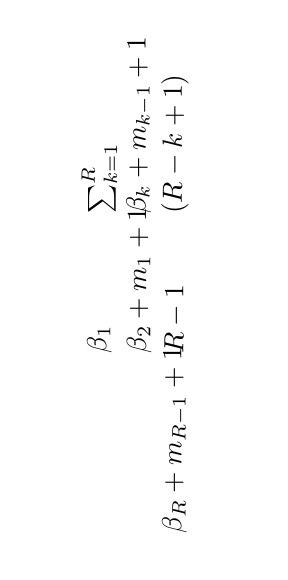
\begin{tikzpicture}[node distance=-.35cm]
\matrix[matrix of nodes,row sep=-.2cm,column sep=.1cm,matrix anchor=north east,outer sep=0pt]{% 
\rule{0pt}{4ex}&% 
\rule{0pt}{3ex}&% 
\multicolumn{1}{c}{\rotatebox{90}{$\sum_{k=1}^R$}}&% 
\multicolumn{1}{c}{\rotatebox{90}{$\beta_k+m_{k-1}+1$}}&% 
\multicolumn{1}{c}{\rotatebox{90}{$(R-k+1)$}}&% 
\rule{0pt}{3ex}&% 
\rule{0pt}{4ex}\\ 
\rule{0pt}{3ex}&% 
\rule{0pt}{3ex}&% 
\multicolumn{1}{c}{\rotatebox{90}{$\beta_1$}}&% 
\multicolumn{1}{c}{\rotatebox{90}{$\beta_2+m_1+1$}}&% 
\multicolumn{1}{c}{\rotatebox{90}{$R-1$}}&% 
\rule{0pt}{3ex}&% 
\rule{0pt}{3ex}\\ 
\rule{0pt}{3ex}&% 
\rule{0pt}{3ex}&% 
\rule{0pt}{3ex}&% 
\rule{0pt}{3ex}&% 
\multicolumn{1}{c}{\rotatebox{90}{$\beta_R+m_{R-1}+1$}}&% 
\rule{0pt}{3ex}&% 
\rule{0pt}{3ex}\\ 
};
\end{tikzpicture}
\end{document}